\chapter{Desenvolvimento do projeto}
\label{chap:metod}
O primeiro passo para o desenvolvimento desse estudo foi a montagem do robô Turtlebot3 e a realização do tutorial disponível no site \cite{ROBOTIS}. Foi instalada a imagem do Ubuntu 20.04 na Raspberry Pi, o ROS Noetic, as dependências necessárias e os pacotes do Turtlebot3 ros-noetic-dynamixel-sdk, ros-noetic-turtlebot3-msgs e o ros-noetic-turtlebot3.

Para implementar o planejador de trajetória PRM foi feita inicialmente uma busca das soluções já disponíveis na internet. Foi encontrado um pacote no GitHub no Link \cite{mwswartwout} que implementa o planejador PRM como Plugin no ROS. O pacote foi desenvolvido para outra versão de ROS, foram necessário fazer algumas modificações no mesmo e também instalar algumas dependências necessárias: occupancy\textunderscore grid\textunderscore utils, ros\textunderscore noetic\textunderscore tf2\textunderscore bullet, ros\textunderscore noetic\textunderscore ompl e ros\textunderscore noetic\textunderscore ompl\textunderscore dbgsym.

No site \url{http://wiki.ros.org/navigation/Tutorials/Writing%20A%20Global%20Path%20Planner%20As%20Plugin%20in%20ROS} é encontrado um tutorial de como desenvolver o planejador como Plugin e como utilizá-lo. 
Para selecionar o PRM como planejador global do Move Base é necessário alterar o parâmetro base\textunderscore global\textunderscore planner do pacote turtlebot3\textunderscore navigation para o PRM.

Foi desenvolvido um repositório no GitHub com o planejador PRM com as modificações e o tutorial de como instalar as dependências necessárias. O repositório se encontra nesse site \url{https://github.com/seixasxbr/prm_planner}.

\section{Simulação}

A simulação do sistema foi realizada no software Gazebo para validar o funcionamento do planejador de trajetórias PRM. A simulação pode ser vista na Figura \ref{fig:simu}.

\begin{figure} [h!]	
    \centering
    \caption{Simulação no Gazebo}
    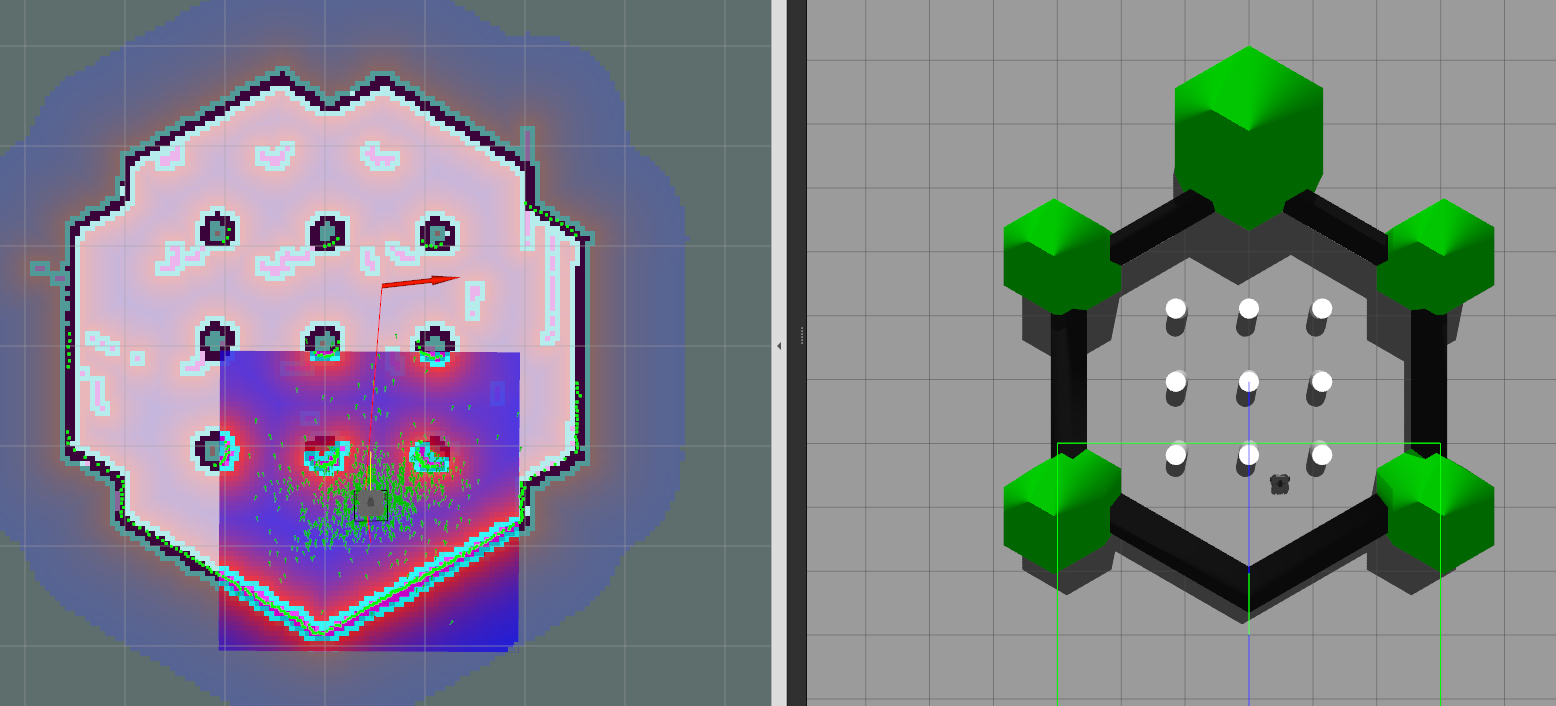
\includegraphics[width=1\textwidth]{Figures/Screenshot from 2021-12-19 12-58-25 (1).png}
    \caption*{Fonte: Autoria própria.}
    \label{fig:simu}
 \end{figure}

\section{Prática}

O planejador foi testado também no mundo real, sendo utilizado um labirinto para avaliar a navegação autônoma do robô utilizando o PRM como planejador global. A foto do experimento pode ser visto na Figura \ref{fig:pratica}.

\begin{figure} [h!]	
    \centering
    \caption{Simulação no Gazebo}
    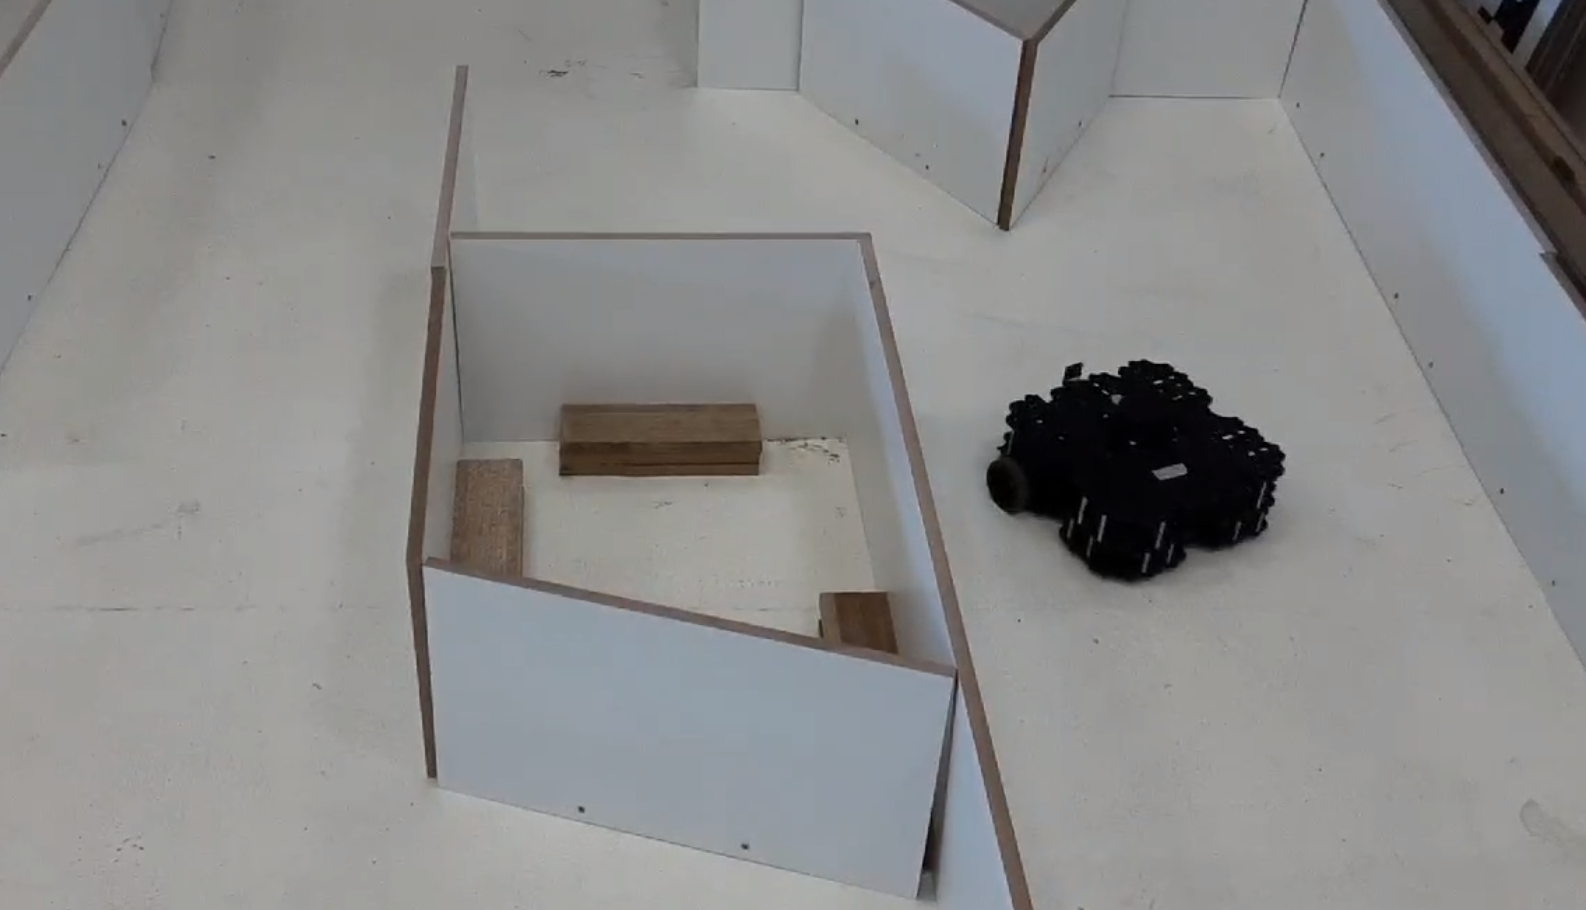
\includegraphics[width=1\textwidth]{Figures/Screenshot from 2021-12-19 13-13-10.png}
    \caption*{Fonte: Autoria própria.}
    \label{fig:pratica}
 \end{figure}